% Created with jtex v.1.0.17
\documentclass{article}
\PassOptionsToPackage{short, nodayofweek}{datetime}


% Start Curvenote Definitions

% Pass Options Section
% base
\PassOptionsToPackage{normalem}{ulem}
\PassOptionsToPackage{utf8}{inputenc}

% template
\PassOptionsToPackage{framemethod=TikZ}{mdframed}
\PassOptionsToPackage{x11names, svgnames}{xcolor}

%%% PACKAGES

% base
\usepackage{inputenc}
\usepackage{url}
\usepackage{graphicx}
\usepackage{adjustbox}
\usepackage{amssymb}
\usepackage{amsfonts}
\usepackage{amsmath}
\usepackage{enumitem}
\usepackage{nicefrac}
\usepackage{booktabs}
\usepackage{microtype}
\usepackage{hyperref}
\usepackage{ulem}
\usepackage{enumitem}
\usepackage{float}
\usepackage{datetime}
\usepackage{xkeyval}
\usepackage{framed}
\usepackage{doi}

% template
\usepackage{natbib}
\usepackage{fancyvrb}
\usepackage{mdframed}
\usepackage{xcolor}

%%%


%%%% Setup Section

% base
\graphicspath{{.}}
% template
\sloppy
\newenvironment{aside}{\begin{framed}}{\end{framed}}
\newmdenv[linewidth=2pt,linecolor=CornflowerBlue,topline=false,bottomline=false,rightline=false,leftline=true,skipabove=20,skipbelow=20,leftmargin=20,rightmargin=20]{callout}
\newfloat{code}{thp}{loc}
\floatname{code}{Program}
\raggedbottom
\bibliographystyle{abbrvnat}
\setcitestyle{authoryear,open={(},close={)},semicolon,aysep={,}}

% End Curvenote Definitions




% colors for hyperlinks
\hypersetup{colorlinks=true, allcolors=blue}
\hypersetup{
pdftitle={\@title},
pdfsubject={},
pdfauthor={\@author},
pdfkeywords={},
addtopdfcreator={Written in Curvenote}
}

\usepackage{curvenote}

\title{EOMAJI scientific background}

\newdate{articleDate}{21}{4}{2024}
\date{\displaydate{articleDate}}

\author{\bfseries Hector Nieto\mdseries\\ICA-CSIC\\\AND\bfseries Benjamin Mary\mdseries\\ICA-CSIC\\\AND\bfseries Vicente Burchard-Levine\mdseries\\ICA-CSIC\\}

\begin{document}

\maketitle
\keywords{DA}

\section{Abstract}

\section{Background and objectives}

% 
% comment
%

Project EOMAJI (Earth Observation system to Manage Africa's food systems by Joint-knowledge of crop production and Irrigation digitization)
ET-Based algoritms for net irrigation estimation.

\subsection{Identifying irrigation events through monitoring of changes in ET}

The \textbf{ratio of actual to potential ET (ETa/p)} should be used in order to avoid changes in ET
due to changes in weather (e.g. increased wind speed) or crop cover (e.g. quick development of
leaves) being attributed to irrigation. This ratio is closely related to root-zone water availability and
therefore is mainly influenced by irrigation or rainfall events.

This is achieved by first calculating the change in \textbf{ETa/p} between the time on which irrigation is to be detect and most recent previous time on which ET estimates are available. This change is \textbf{calculated both locally (i.e. at individual pixel level) and regionally} (i.e. as an average change in all agricultural pixels within 10 km window).

The local and regional changes are then \textbf{compared to a number of thresholds} to try to detect if:

\begin{itemize}
\item a) There is no input of water into the soil (e.g. local ETa/p does not increase above a threshold)
\item b) There is input of water into the soil but due to rainfall (e.g. increase in regional ETa/p is over a
threshold and larger or similar to increase in local Eta/p)
\item c) There is input of water to the soil due to irrigation (e.g. increase in local ETa/p is over a
threshold and significantly larger than increase in regional ETa/p)
\end{itemize}

Detected irrigation events are further split into \textbf{low, medium and high probability} based on another set
of thresholds. Since irrigation is normally applied on a larger area, the raster map with per-pixel
irrigation events is cleaned up by removing isolated pixels in which irrigation was detected.

\begin{figure}[!htbp]
\centering
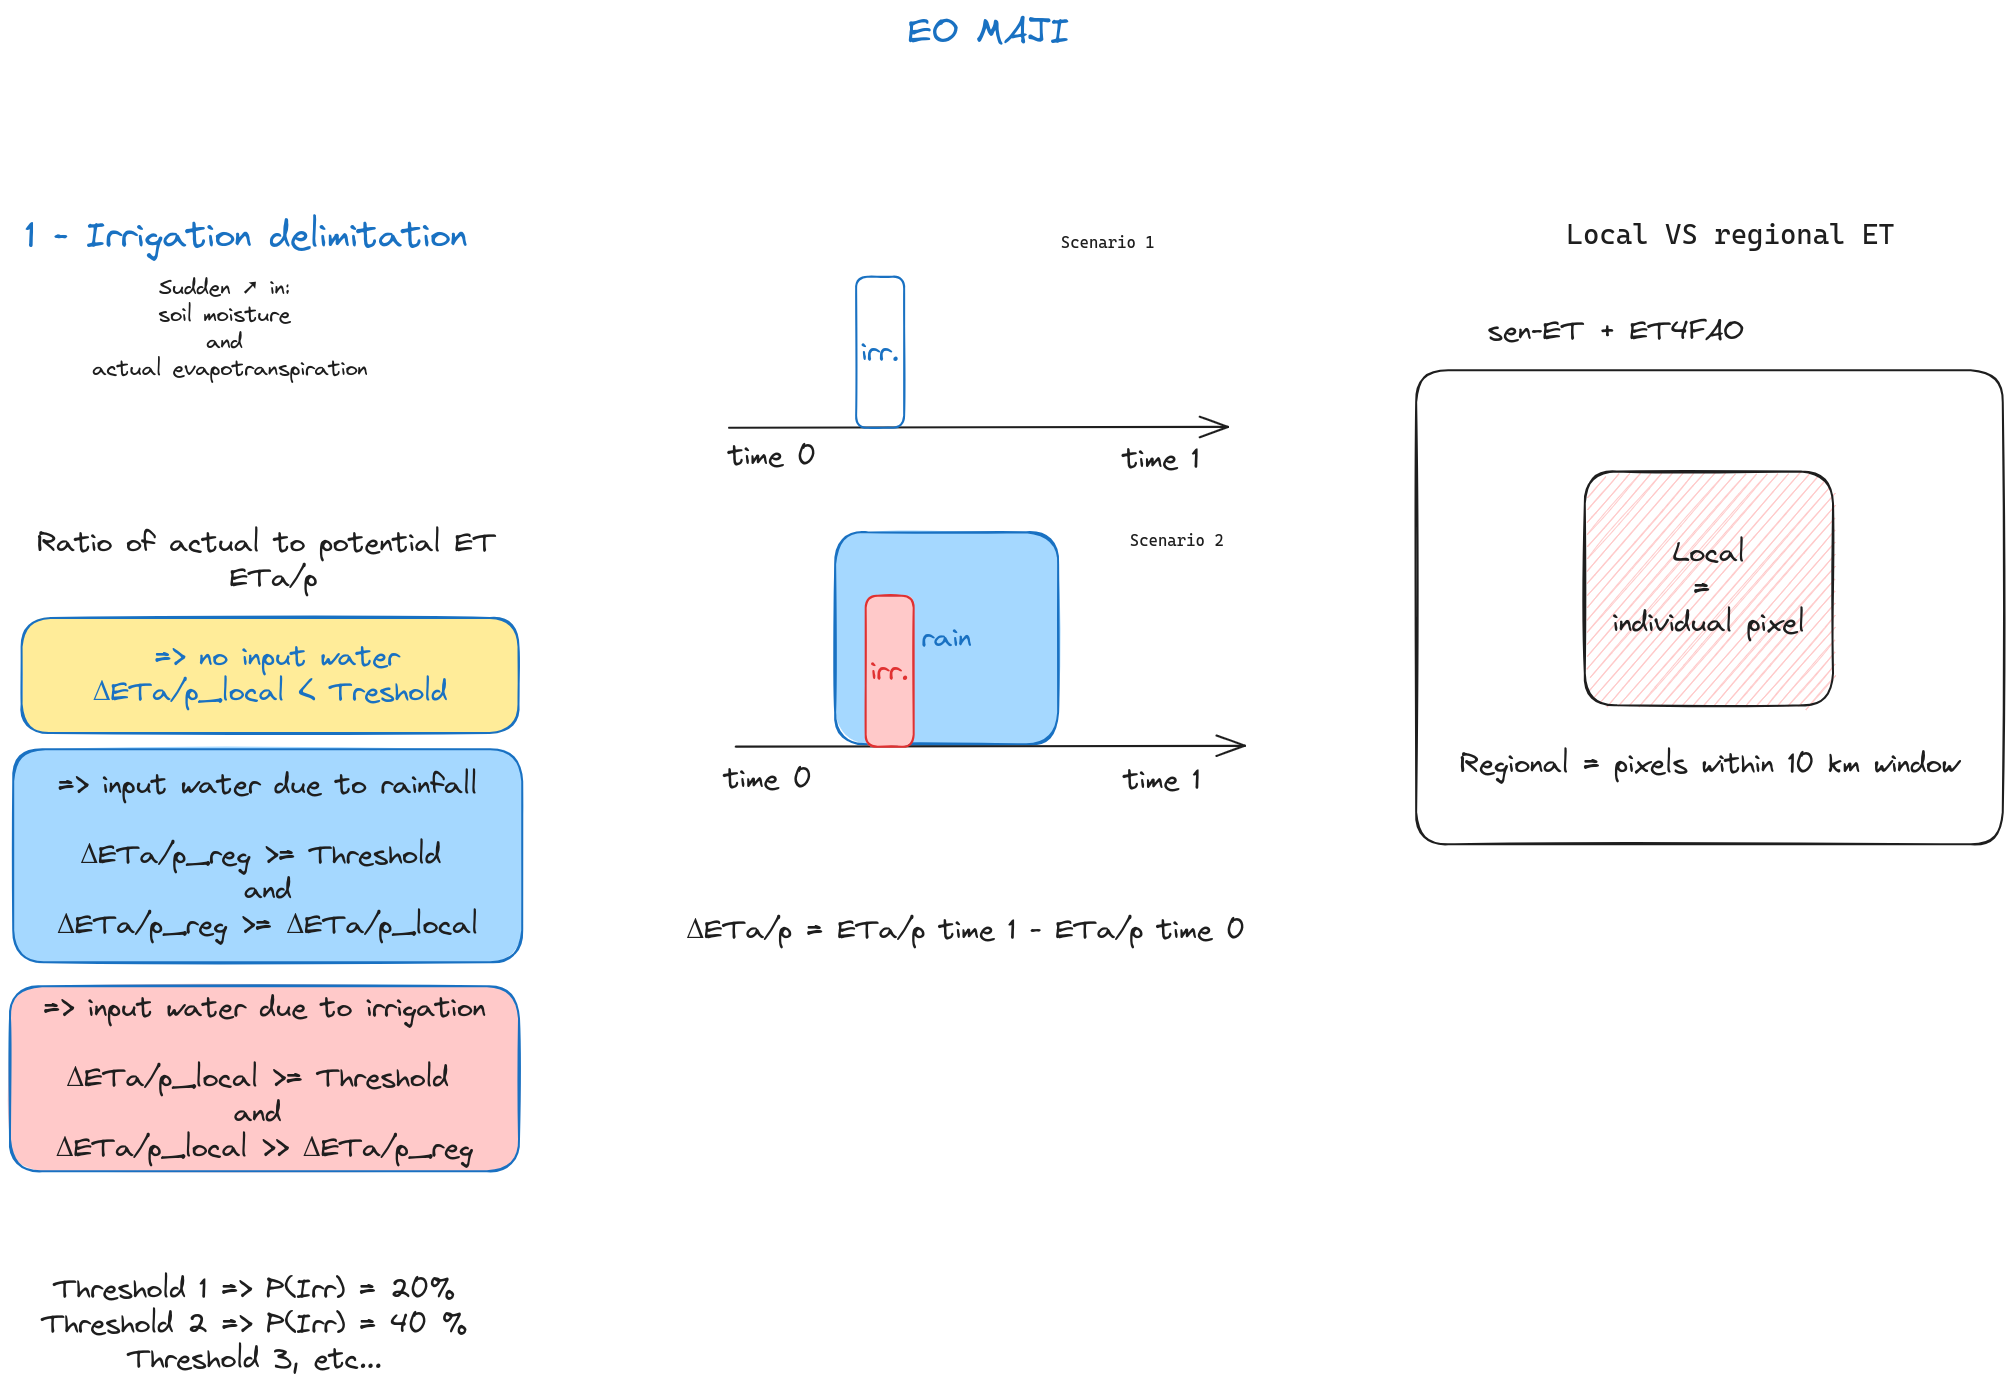
\includegraphics[width=0.375\linewidth]{files/EO-MAJI-IrrDelineati-f37af6d89c8d3154757841641d758e25.png}
\caption*{EO-MAJI-IrrDelineation}
\end{figure}

\begin{figure}[!htbp]
\centering
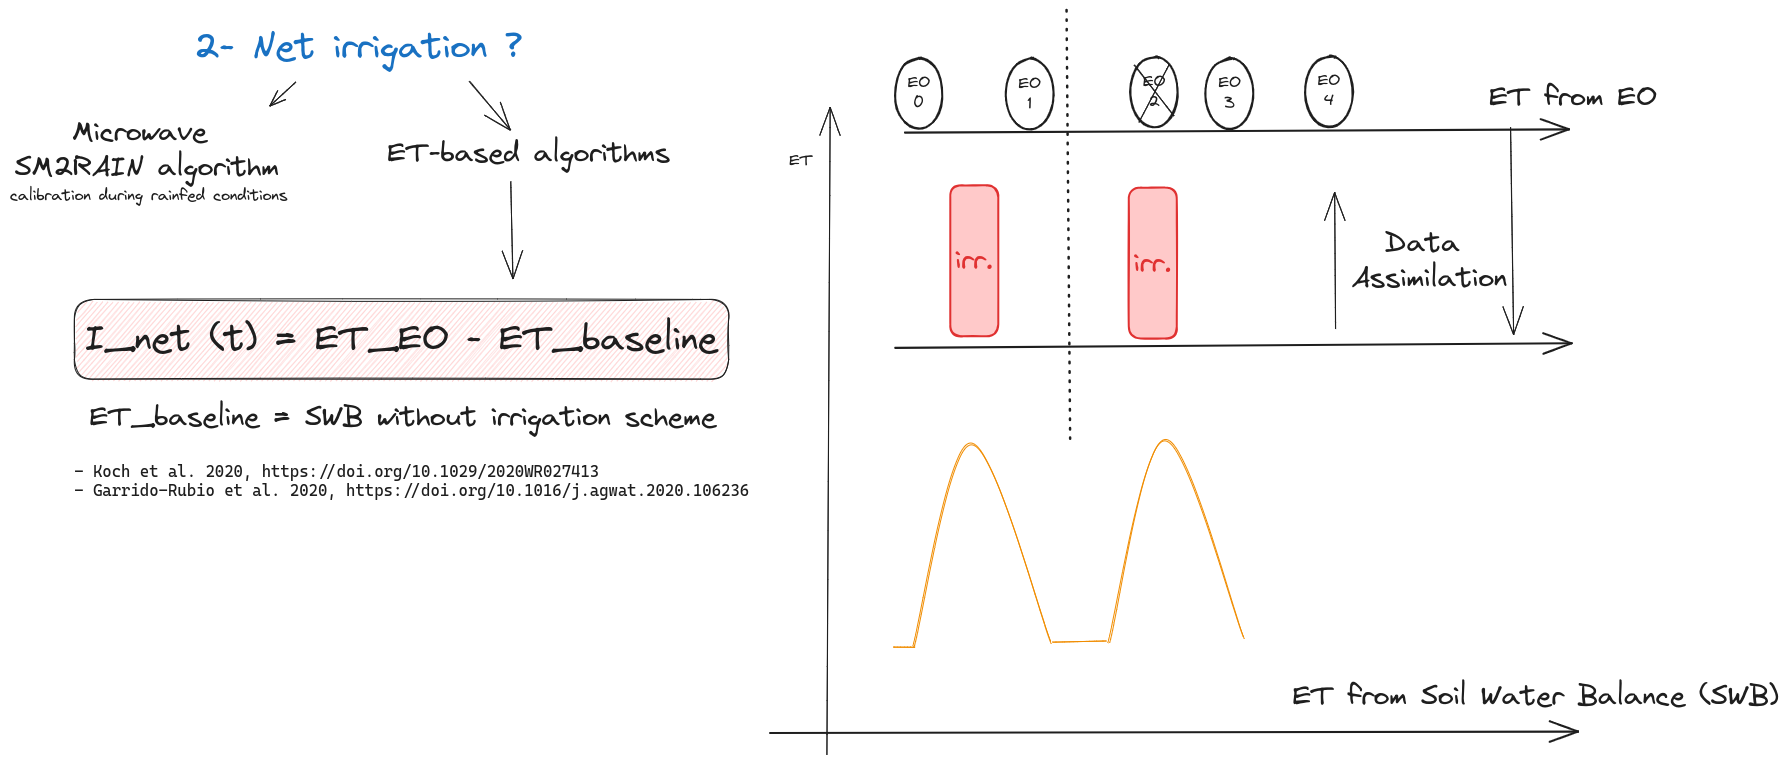
\includegraphics[width=0.375\linewidth]{files/EO-MAJI-IrrNet-3a015ba044e67d3d0d8460677742b6be.png}
\caption*{Issue with rain event}
\end{figure}

\subsection{Quantifying irrigation}

Inet\_EOMAJI

\begin{figure}[!htbp]
\centering
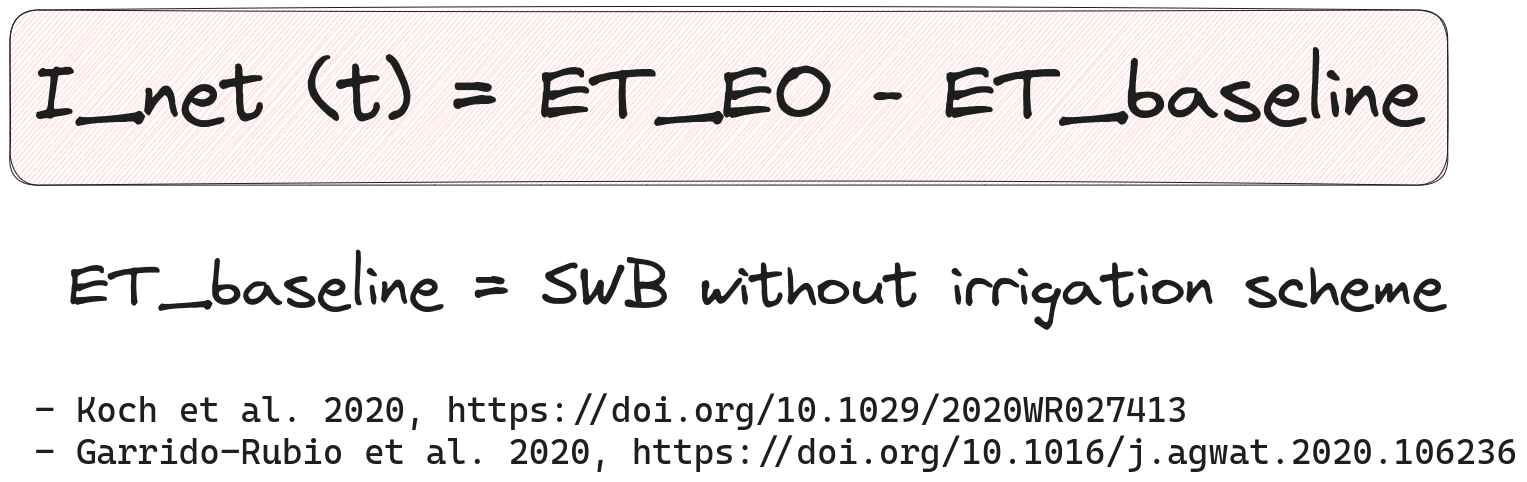
\includegraphics[width=0.75\linewidth]{files/Inet_EOMAJI-c4b87b879641d93a98c453dcee2215b6.png}
\caption*{EO-MAJI-Inet}
\end{figure}
\end{document}
